%\title{LaTeX Portrait Poster Template}
%%%%%%%%%%%%%%%%%%%%%%%%%%%%%%%%%%%%%%%%%
% a0poster Portrait Poster
% LaTeX Template
% Version 1.0 (22/06/13)
%
% The a0poster class was created by:
% Gerlinde Kettl and Matthias Weiser (tex@kettl.de)
% 
% This template has been downloaded from:
% http://www.LaTeXTemplates.com
%
% License:
% CC BY-NC-SA 3.0 (http://creativecommons.org/licenses/by-nc-sa/3.0/)
%
%%%%%%%%%%%%%%%%%%%%%%%%%%%%%%%%%%%%%%%%%

%----------------------------------------------------------------------------------------
%	PACKAGES AND OTHER DOCUMENT CONFIGURATIONS
%----------------------------------------------------------------------------------------
\documentclass[a0,portrait]{a0poster}

\usepackage{multicol} % This is so we can have multiple columns of text side-by-side
\columnsep=100pt % This is the amount of white space between the columns in the poster
\columnseprule=3pt % This is the thickness of the black line between the columns in the poster

\usepackage[svgnames]{xcolor} % Specify colors by their 'svgnames', for a full list of all colors available see here: http://www.latextemplates.com/svgnames-colors

\usepackage{times} % Use the times font
%\usepackage{palatino} % Uncomment to use the Palatino font

\usepackage{graphicx} % Required for including images
\graphicspath{{figures/}} % Location of the graphics files
\usepackage{booktabs} % Top and bottom rules for table
\usepackage[font=large,labelfont=bf]{caption} % Required for specifying captions to tables and figures
\usepackage{amsfonts, amsmath, amsthm, amssymb} % For math fonts, symbols and environments
\usepackage{wrapfig} % Allows wrapping text around tables and figures

\definecolor{light-gray}{gray}{0.9}
\newcommand{\code}[1]{\colorbox{light-gray}{\texttt{#1}}}

\usepackage{amsmath}
\usepackage[linesnumbered,ruled]{algorithm2e}

\usepackage[export]{adjustbox}

\usepackage{array}

\begin{document}

%----------------------------------------------------------------------------------------
%	POSTER HEADER 
%----------------------------------------------------------------------------------------

% The header is divided into two boxes:
% The first is 75% wide and houses the title, subtitle, names, university/organization and contact information
% The second is 25% wide and houses a logo for your university/organization or a photo of you
% The widths of these boxes can be easily edited to accommodate your content as you see fit

\begin{minipage}[b]{0.80\linewidth}
\veryHuge \color{NavyBlue} \textbf{Genetic Analysis via Iterative Hard-Thresholding}\\ \color{Black} % Title
\Huge\textit{Collab with Open Mendel using the Julia programming language}\\[2cm] % Subtitle
\huge \textbf{Benjamin Chu \& Kevin Keys \& Janet Sinsheimer \& Kenneth Lange}\\[0.5cm] % Author(s)
\huge Department of Biomathematics\\[0.4cm]
\normalsize 
Contacts: \texttt{biona001@ucla.edu, kevin.keys@ucsf.edu, JanetS@mednet.ucla.edu,  klange@ucla.edu} \\
Repository: \texttt{https://github.com/klkeys/IHT.jl} \\
\end{minipage}
%
\begin{minipage}[b]{0.25\linewidth}
\centering
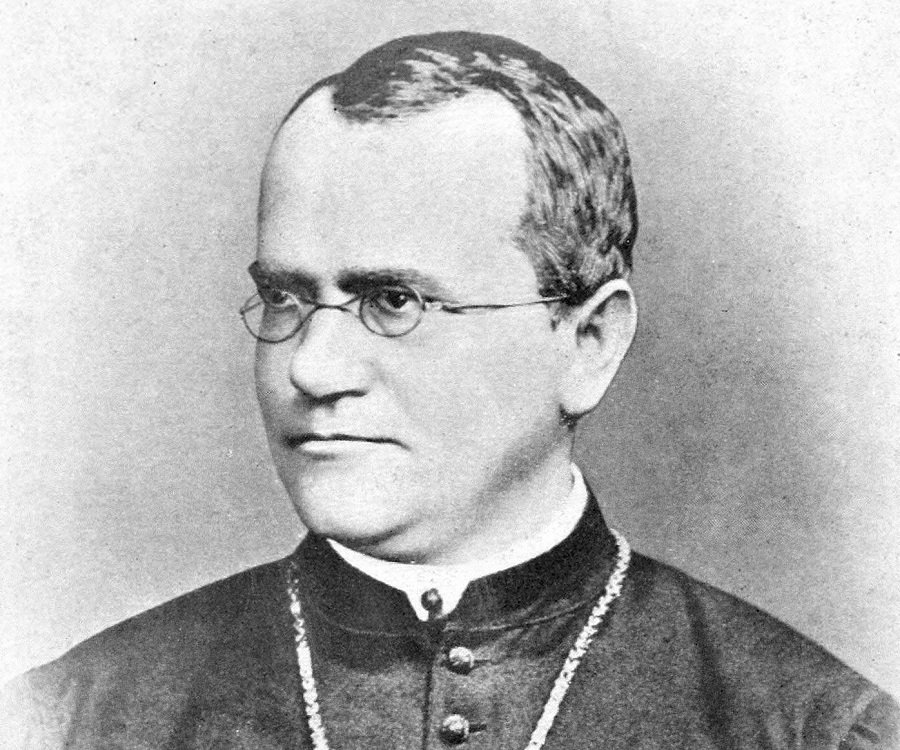
\includegraphics[width=12cm]{figures/gregor-mendel-3.jpg}

\includegraphics[width=15cm]{figures/ucla-std-blu-cmyk.jpg}
\end{minipage}

%\vspace{1cm} % A bit of extra whitespace between the header and poster content

%----------------------------------------------------------------------------------------

\begin{multicols}{2} % This is how many columns your poster will be broken into, a portrait poster is generally split into 2 columns

\color{Navy} % Navy color for the abstract
\section*{Background - Some Problems in Statistical Genetics}

\color{Black} % Navy color for the abstract

\raggedright
At the DNA level, modern humans are 99.9\% identical. The remaining 0.1\% of genetic variations drive many trait and disease differences observed in humans. Individual variations in the DNA sequence are termed \textbf{single nucleotide polymorphisms} (SNPs) and biologists can identify them via \textbf{Genome Wide Association Studies} (GWAS). These studies aim to answer one main question:

\vspace{1cm}
\centering \Large \textbf{Q: Which genetic variants are associated with a trait?}

\raggedright \normalsize
\subsection*{A few Obstacles...}
\begin{itemize}
	\item GWAS datasets are often \textbf{super big} (100+ GB). \textbf{\color{Green} Q: How to analyze them efficiently? } \color{black}
	\item SNPs are often \textbf{rare} with \textbf{small effect size}. \color{Green} \textbf{Q: How to separate \textit{weak signals} from \textit{noise}}?  \color{black}
	\item Genetic data processing is \textbf{unnecessarily complicated}.\color{Green} \textbf{ Q: Can we not have a centralized platform providing a streamlined pipeline for genetic analysis?} \color{black}
\end{itemize}

\color{Navy} % Navy color for the abstract

\section*{Features of IHT.jl}

\color{Black} % SaddleBrown color for the introduction
\begin{enumerate}
	\item \textbf{Integration with Open Mendel:} Prepare 1 input file to not only run IHT, but also 11 more genetics analyses, such as simulation, fitting variance component model, linkage analysis...etc
	\item \textbf{Doubly sparse group projection:} Optionally estimates sparse $\beta$ with at most $J$ active groups and $k$ active predictors per group. 
	\item \textbf{Scale SNPs using prior weights:} User can optionally scale each SNP's weight based on known information (frequency, data quality, candidate gene/pathway approach...etc)
	\item \textbf{GPU acceleration(*):} Greatly improves computational performance (only for numeric data).
	\item \textbf{Cross Validation(*):} Automatically determines optimal number of features\\
	\vspace{0.5cm}
	\centering (*) $=$ \textit{only available when interfacing with PLINK.jl $=$ future work}
\end{enumerate}



\color{Navy} % Navy color for the abstract

\section*{Key Performance Optimizations}

\color{Black} % SaddleBrown color for the introduction
\begin{itemize}
	\item \textbf{Computation on raw genotypes.} IHT.jl interfaces with SnpArrays.jl to perform the following linear algebra directly on raw genotype data: \code{A\_mul\_B!}, \code{At\_mul\_B!}, \code{A\_mul\_Bt!}, \code{At\_mul\_Bt!}, \code{Ac\_mul\_B!}, \code{A\_mul\_Bc!}, \code{Ac\_mul\_Bc!}. For suitably sized matrices, these routines are faster than analogous BLAS routines because they avoid file swapping with the hard disk (see Figure 2).
\item \textbf{Standardization on the fly.} We can precompute mean minor allele count vector $(\mathbf{u})$ and reciprocal normalizing constant vector $(\mathbf{v})$. Then perform matrix/vector computations directly as:
	\begin{align*}
		\mathbf{X}_{standardized} = \left(\mathbf{X}_{raw} - \mathbf{1}_{n} \mathbf{u}^T\right) diag(\mathbf{v})
	\end{align*}
\item \textbf{Streaming only necessary columns of genotypes.} At each iteration, the estimate of $\beta$ is sparse with none-zero entries denoted by $\beta_k$, and corresponding columns of $\mathbf{X}$ denoted by $\mathbf{X}_k$. Multiplying the 0 entries of $\beta$ with dense $\mathbf{X}$ is redundant. Therefore, we have:
	\begin{align*}
		\nabla f(\beta) = -\mathbf{X}^T(\mathbf{y} - \mathbf{X}\beta) = -\mathbf{X}^T(\mathbf{y} - \mathbf{X}_k\beta_k) 
	\end{align*}
    \item \textbf{Multi-threaded geno-matrix computation (future work)} To speed up the gradient computation, we can make our matrix/vector multiplication multi-threaded. That will be done in the near future.
\end{itemize}

%----------------------------------------------------------------------------------------
%	Math
%----------------------------------------------------------------------------------------

\color{Navy} 
\section*{(Group) Iterative Hard-Thresholding}

\color{Black}

Iterative hard-thresholding (IHT) is one of the most scalable algorithms for \textit{feature selection.} It has great convergence guarantees, and empirically performs better than LASSO and MCP for genetic and numeric data [Keys 2017] in terms of model selection. Below we outline the algorithm and discuss our theoretical contributions.

%------------------------------------------------
\subsection*{Mathematical Section}

For continuous phenotype $\mathbf{Y}$, iterative hard-thresholding minimizes the residual sum of squares subject to different (non-convex) $l_0$ "norm" constraints:

\begin{equation}
f(\beta) = \frac{1}{2}||\mathbf{y} - \mathbf{X}\beta||^2_2, \quad \text{subject to} 
\begin{cases}
  \text{Regular IHT:} \ &||\beta||_0 \leq k\\
  \text{Group IHT:} \ &||G_i(\beta)||_0 \leq k, \quad i \in \{1,...,J\}
\end{cases}
\end{equation}

The sparsity constraints $k, J$ and group memberships $G$ are assumed to be known, but in practice they have to be determined via cross-validation. Note that when $J = 1$, group IHT reduces to regular IHT. Update to $\beta$ is accomplished \textit{iteratively} by first taking the negative gradient step, then project so at most $J$ active groups and $k$ active predictors per group remains:

\begin{eqnarray}
\beta^+ = P_{S_{J, k}} \left[\beta - \mu \nabla f(\beta) \right], \quad \mu_m = \frac{||\beta^m||^2_2}{||X\beta^m||^2_2}\label{edgek}
\end{eqnarray}
The operator $P_{S_{J,k}}$ finds the $J$ largest group in $l_2$ magnitude first, leaves the $k$ largest entry of each group alone, and sets everything else to $0$. For normal IHT, convergence is guaranteed if $\mu_m \leq \omega_m$ where:
\begin{eqnarray}
\omega_m \leq (1 - c) \frac{||\beta^{m+1} - \beta^m||_2^2}{||X(\beta^{m+1} - \beta^m)||_2^2}
\end{eqnarray} 
for some constant $0 < c \ll 1$.

\vspace{1cm}

\begin{algorithm*}[H]
    \SetKwInOut{Input}{Input}
    \SetKwInOut{Output}{Output}

    \Input{genotype matrix $\mathbf{X}$, response vector $\mathbf{y}$, membership indicator vector $\mathbf{G}$, scalars $J, k$}
    \Output{$\beta$ with at most $J$ active groups and $k$ active predictors per group}
    \textbf{Initialize:} $\beta \equiv \mathbf{0}.$\\
    
    \While{not converged}
      {
        \textbf{Gradient step:} $\tilde{\beta} = \beta^m - \mu \nabla f(\beta)$\\
        \textbf{Projection:} $\beta^{m+1} = P_{S_{J, k}}(\tilde{\beta})$\\
        \textbf{(Optional) Debiasing}: $\beta^{m+1} = \arg \min f(\beta^{m+1})$ such that $supp(\beta^{m+1})$ satisfies constraints described in (1)
      }
    \caption{(Group) Iterative hard-thresholding}
\end{algorithm*}

%----------------------------------------------------------------------------------------
%	RESULTS 
%----------------------------------------------------------------------------------------

\color{Navy}
\begin{center}
\section*{Results}
\end{center}
\color{Black}

\begin{itemize}
	\item IHT recovers predictors that passes the Bonferroni correction under the scheme of univariate analysis, but also proposes additional predictors that does not pass the cutoff.
	\item Predictors \textbf{might not} be picked even though it has a higher p-value.
	\item On a dataset with 2200 people and 10000 SNPs (roughly 200MB uncompressed), IHT with J = 1 and k = 10 converges in 1.511 seconds and uses 10.5 MB.
\end{itemize}

\vspace{1cm}

\textbf{Future goals:} Enable analysis on half a million samples, whose data size is roughly between 30GB and 1TB. Afterwards, we will focus on proving convergence guarantees for doubly sparse projection and enabling logistic IHT. 

\begin{center}\vspace{1cm}
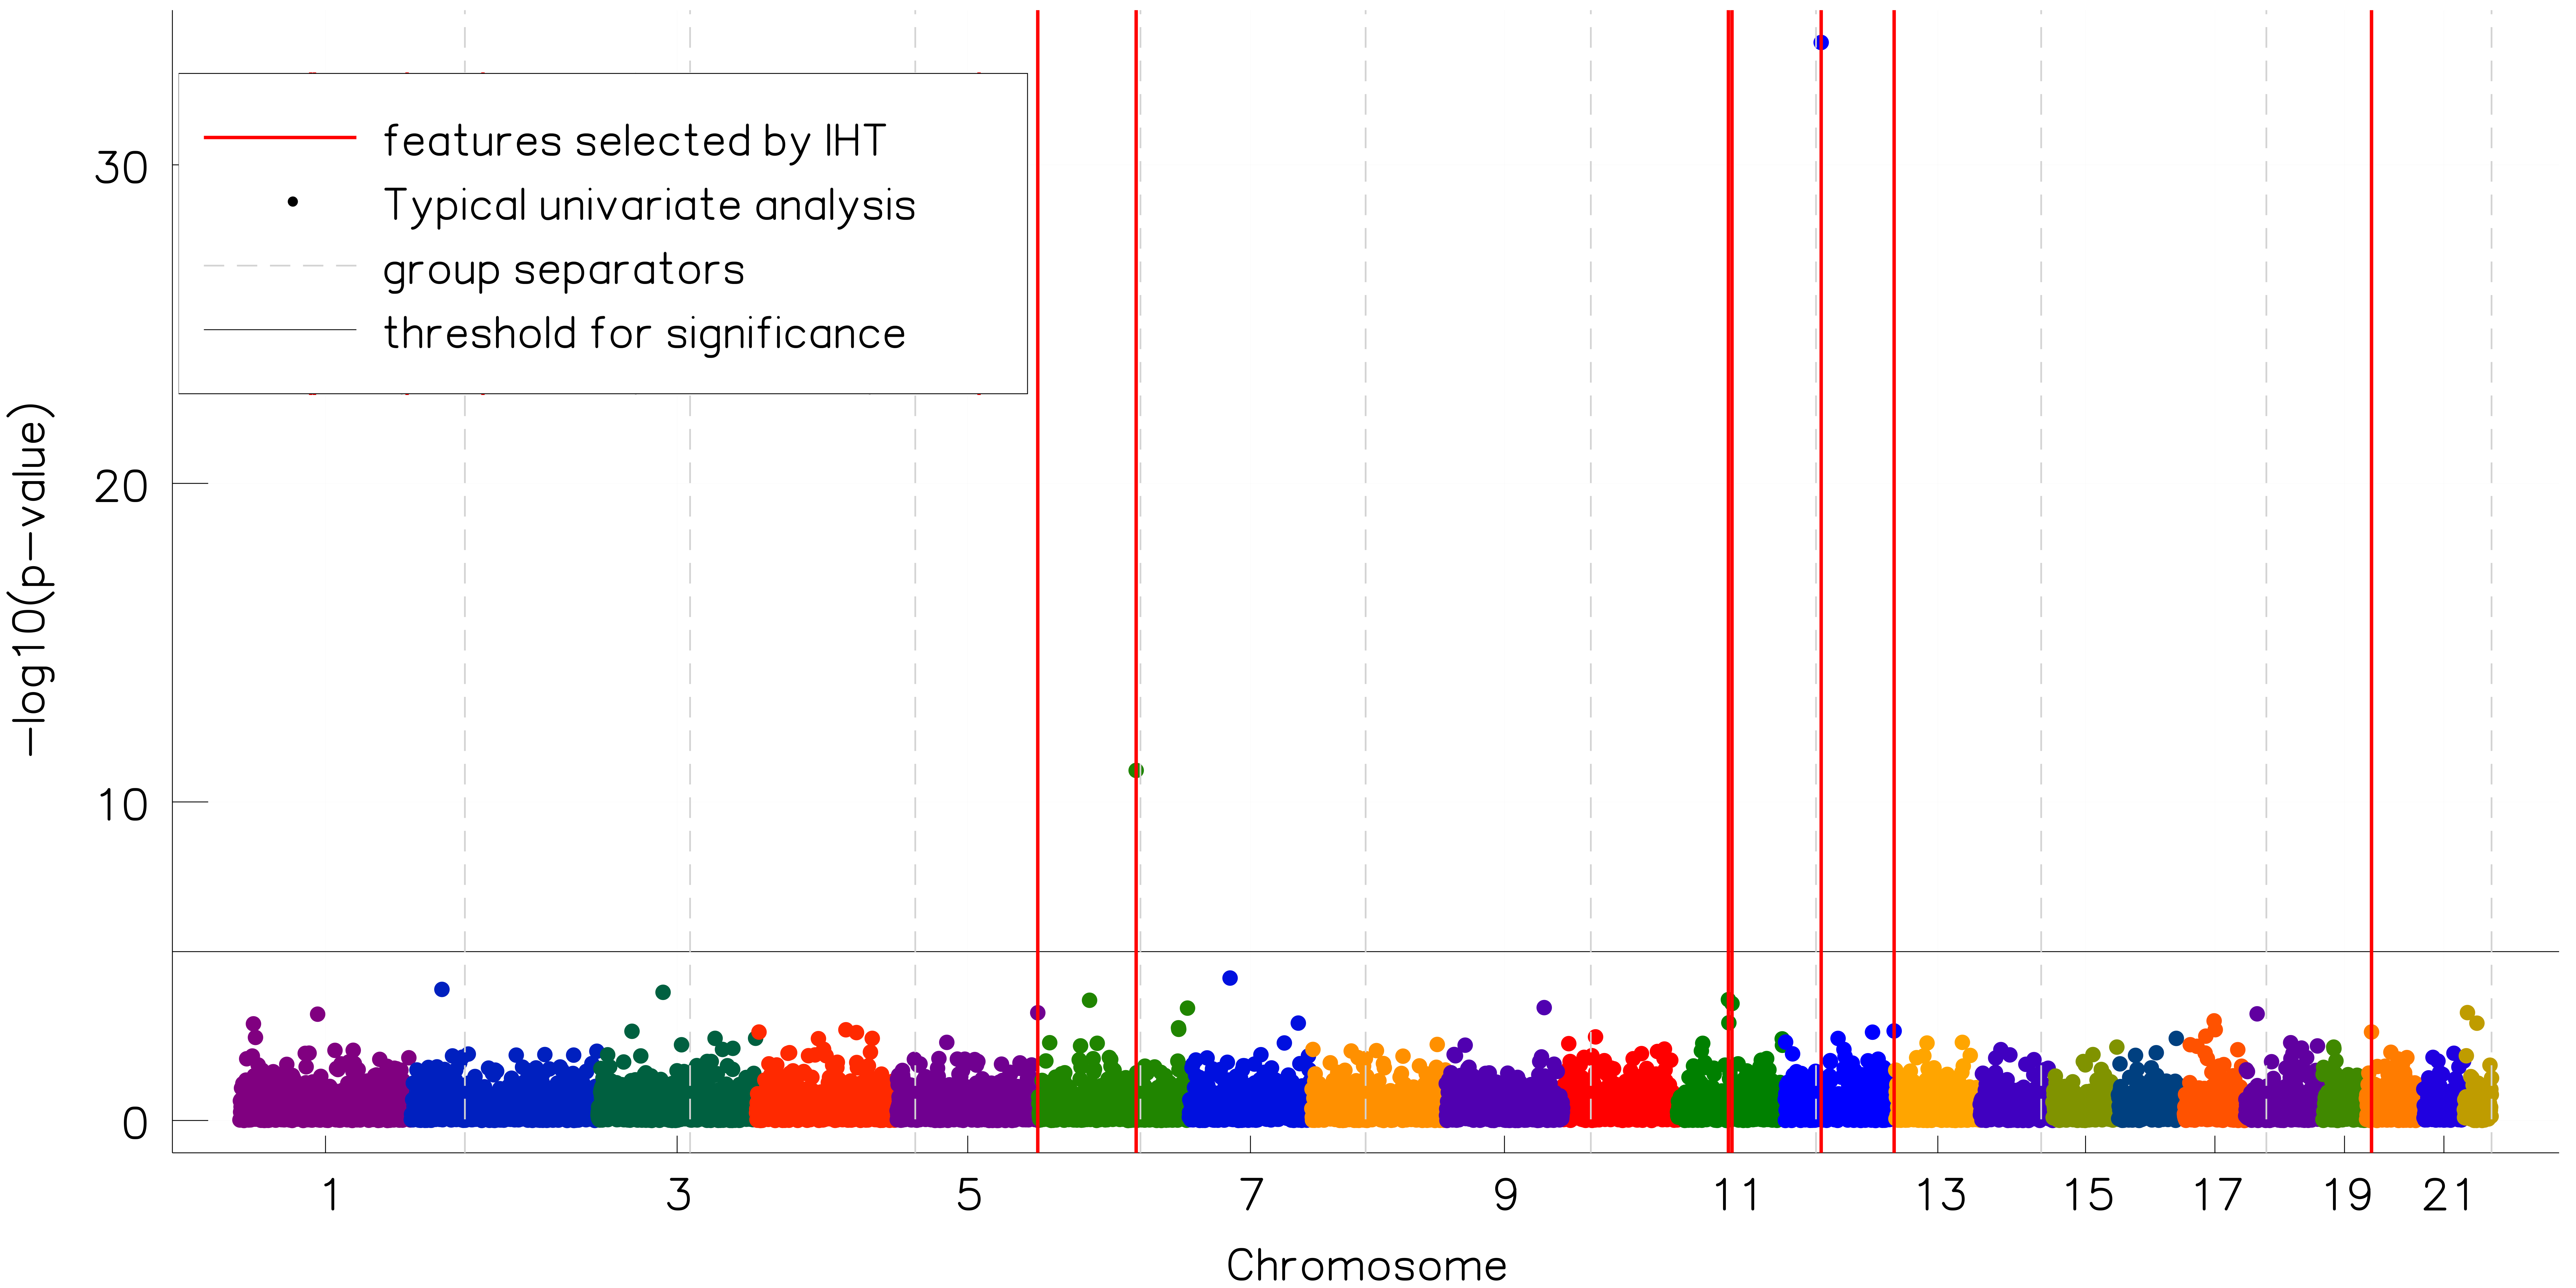
\includegraphics[width=0.9\linewidth]{figures/gwas_1.png}
\captionof{figure}{\color{Green} \textbf{IHT (J=4, k=2) Superimposed on Traditional p-value Graph}}
\end{center}\vspace{1cm}

Table 2 lists a few milestones of our package tested on a 200 MB (uncompressed) dataset:

\vspace{0.5cm}
\begin{center}
\begin{tabular}{c c c c}
\toprule
\textbf{Date} & \textbf{Speed} & \textbf{Memory} & \textbf{Key  improvement}\\
\midrule
June 24 & 1.896 s & 573.3 MB & Prototype code; converts genotype data to float64 matrix\\
July 4 & 2.579 s & 1.230 GB & removed StatsBase dependency, added extra functions\\
July 18 & 2.207 s & 244.1 MB & Enabled matrix subsetting, compute on raw data\\
July 20 & 1.511 s & 10.50 MB & Wrote efficient std computation\\
\bottomrule
\end{tabular}
\end{center}
\vspace{1.5cm}

Figure 2 below compares matrix-vector multiplication speed of BLAS and SnpArrays. For big enough matrices, SnpArrays is faster:

\begin{center}\vspace{1cm}
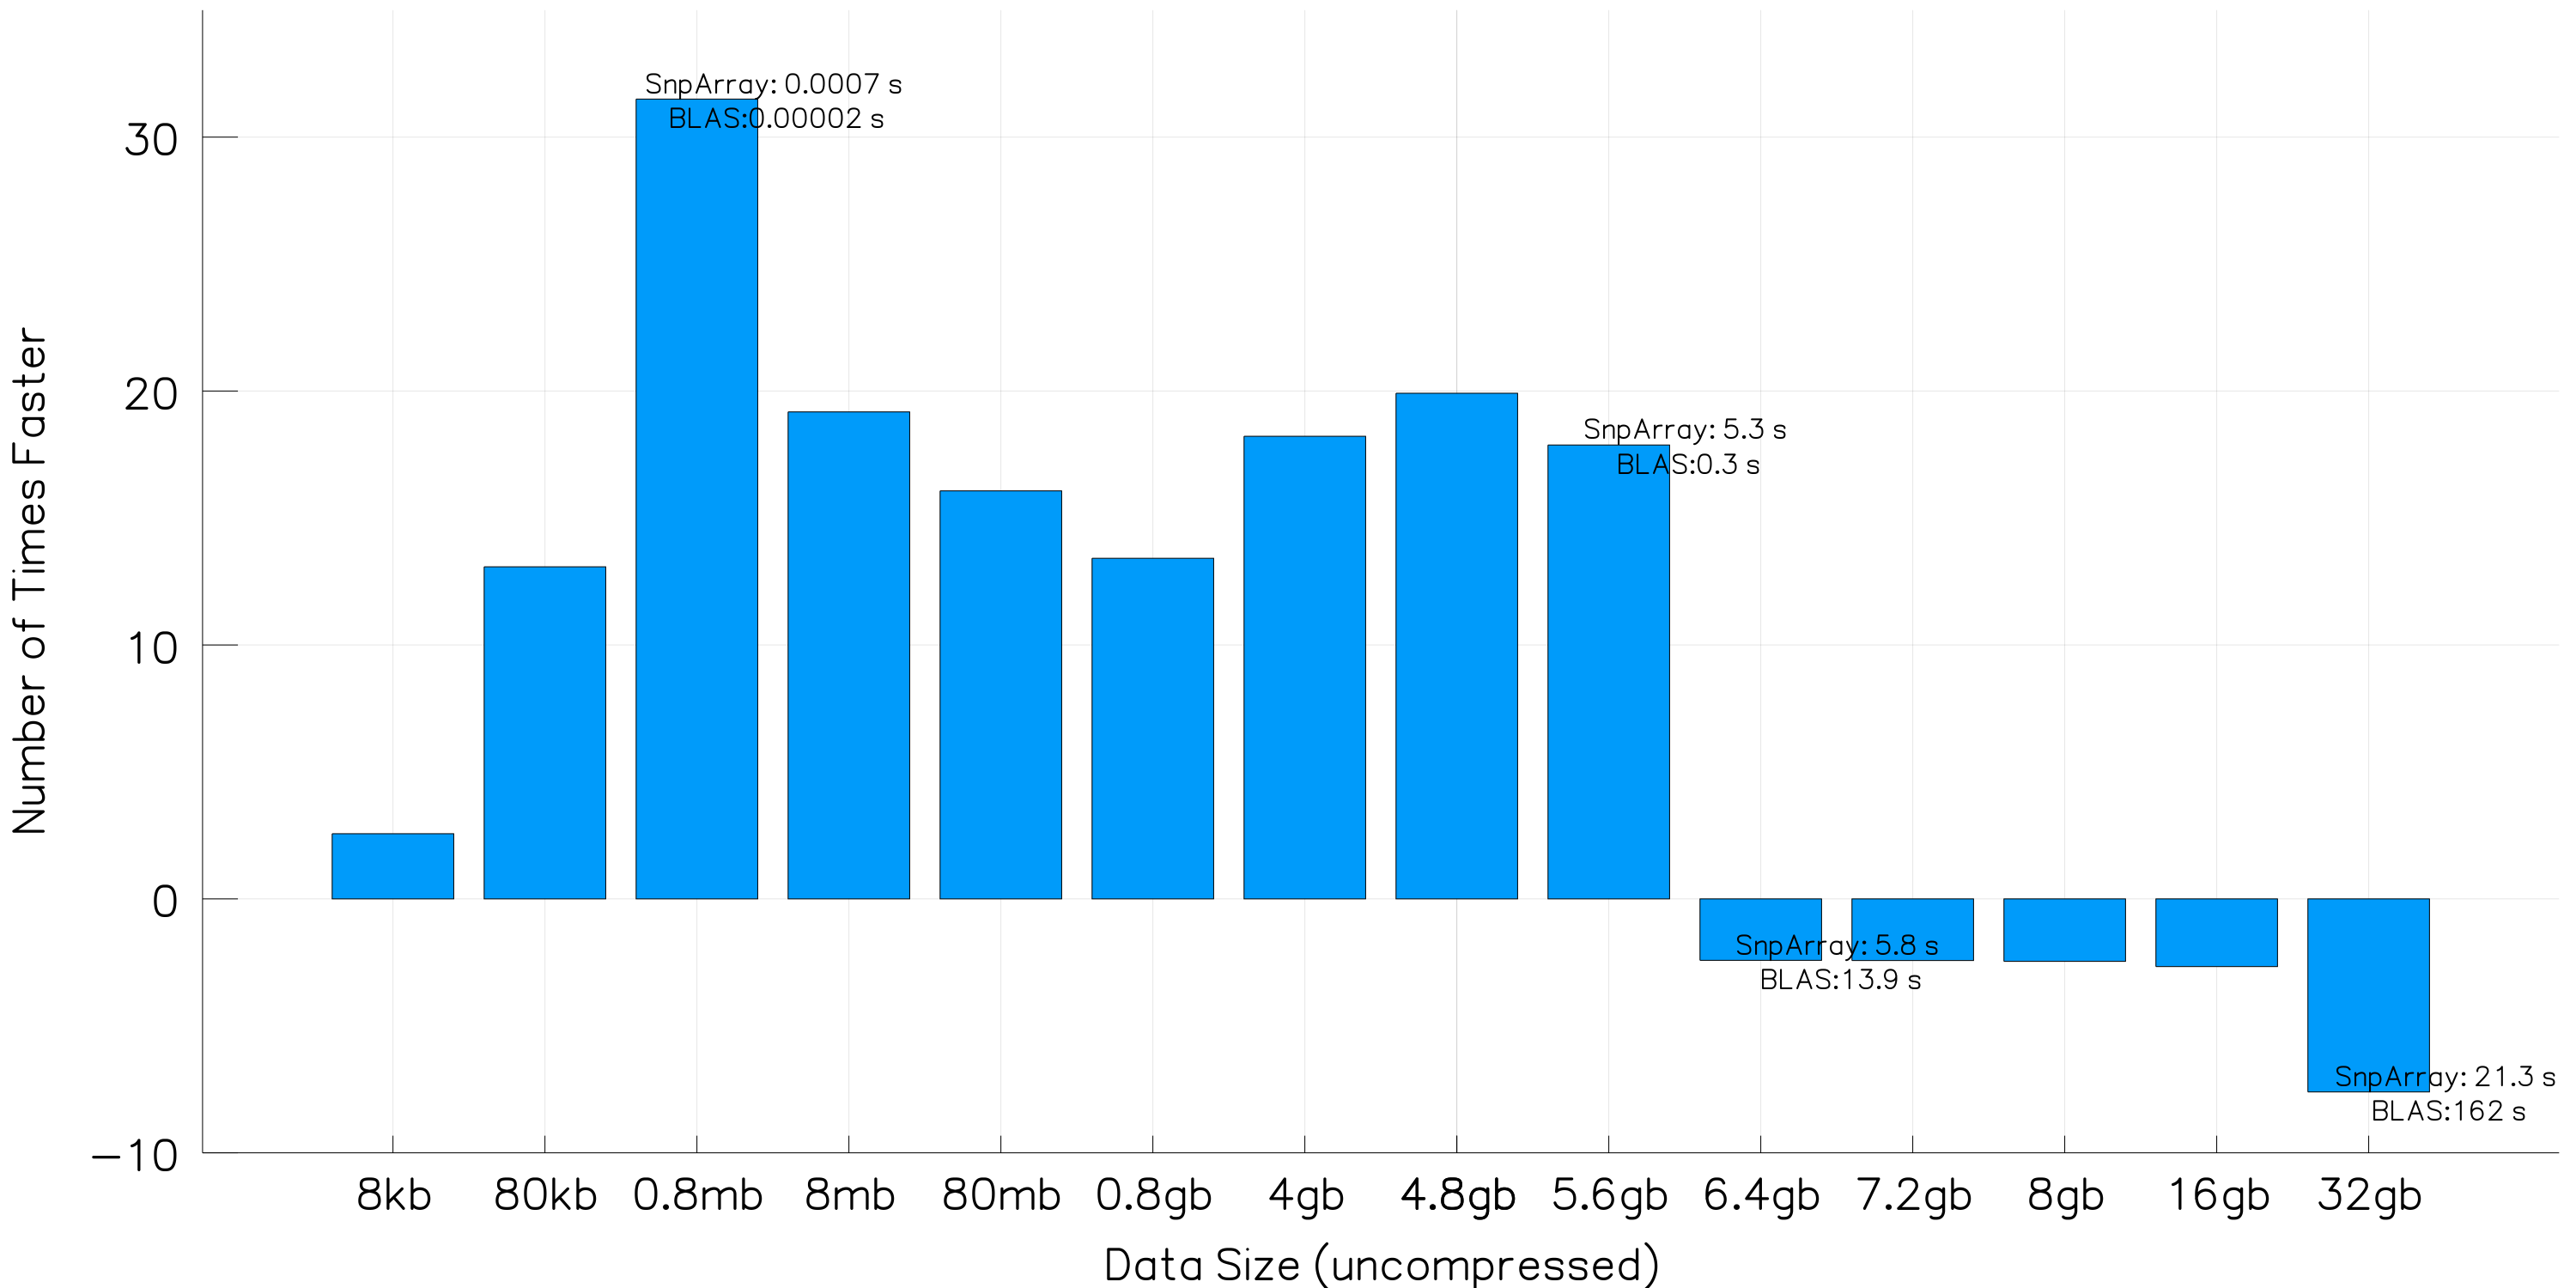
\includegraphics[width=0.9\linewidth]{figures/compare.png}
\captionof{figure}{\color{Green} \textbf{Linear Algebra in SnpArrays is faster than BLAS for Large Matrices}}
\end{center}\vspace{1cm}


%----------------------------------------------------------------------------------------
%	ACKNOWLEDGEMENTS
%----------------------------------------------------------------------------------------
\centering
\color{Navy}
\section*{Acknowledgements}
\color{Black}
\begin{itemize}
\item This research was supported by NIH Training Grant in Genomic Analysis and Interpretation T32HG002536
\item This research was supported by Google Summer of Code 2018 with NumFOCUS.
\item This trip was sponsored by Julia Computing.
\item Special thanks to Kevin Keys for being the best mentor!\end{itemize}
%----------------------------------------------------------------------------------------

\end{multicols}
\end{document}